\documentclass[border=8pt]{standalone}
\usepackage[dvipsnames,svgnames]{xcolor}
\usepackage{amsmath}
\usepackage{amssymb}
\usepackage{tikz}
\usetikzlibrary{
  arrows.meta,
  positioning,
  calc,
  fit,
  backgrounds,
  decorations.pathreplacing,
  shapes.geometric,
  shadows.blur
}
 
% ── colour palette ──────────────────────────────────────────
\definecolor{monoHead}{HTML}{1B3A5C}
\definecolor{monoStage}{HTML}{3A7CA5}
\definecolor{monoLight}{HTML}{D6EAF5}
\definecolor{tfHead}{HTML}{5C3A1B}
\definecolor{tfStage}{HTML}{C47D2B}
\definecolor{tfLight}{HTML}{FAEBD7}
\definecolor{varColor}{HTML}{C0392B}
\definecolor{fixColor}{HTML}{1A7A4C}
\definecolor{bracketGray}{HTML}{555555}
\definecolor{bgLeft}{HTML}{EBF2FA}
\definecolor{bgRight}{HTML}{FDF5EB}
 
\begin{document}
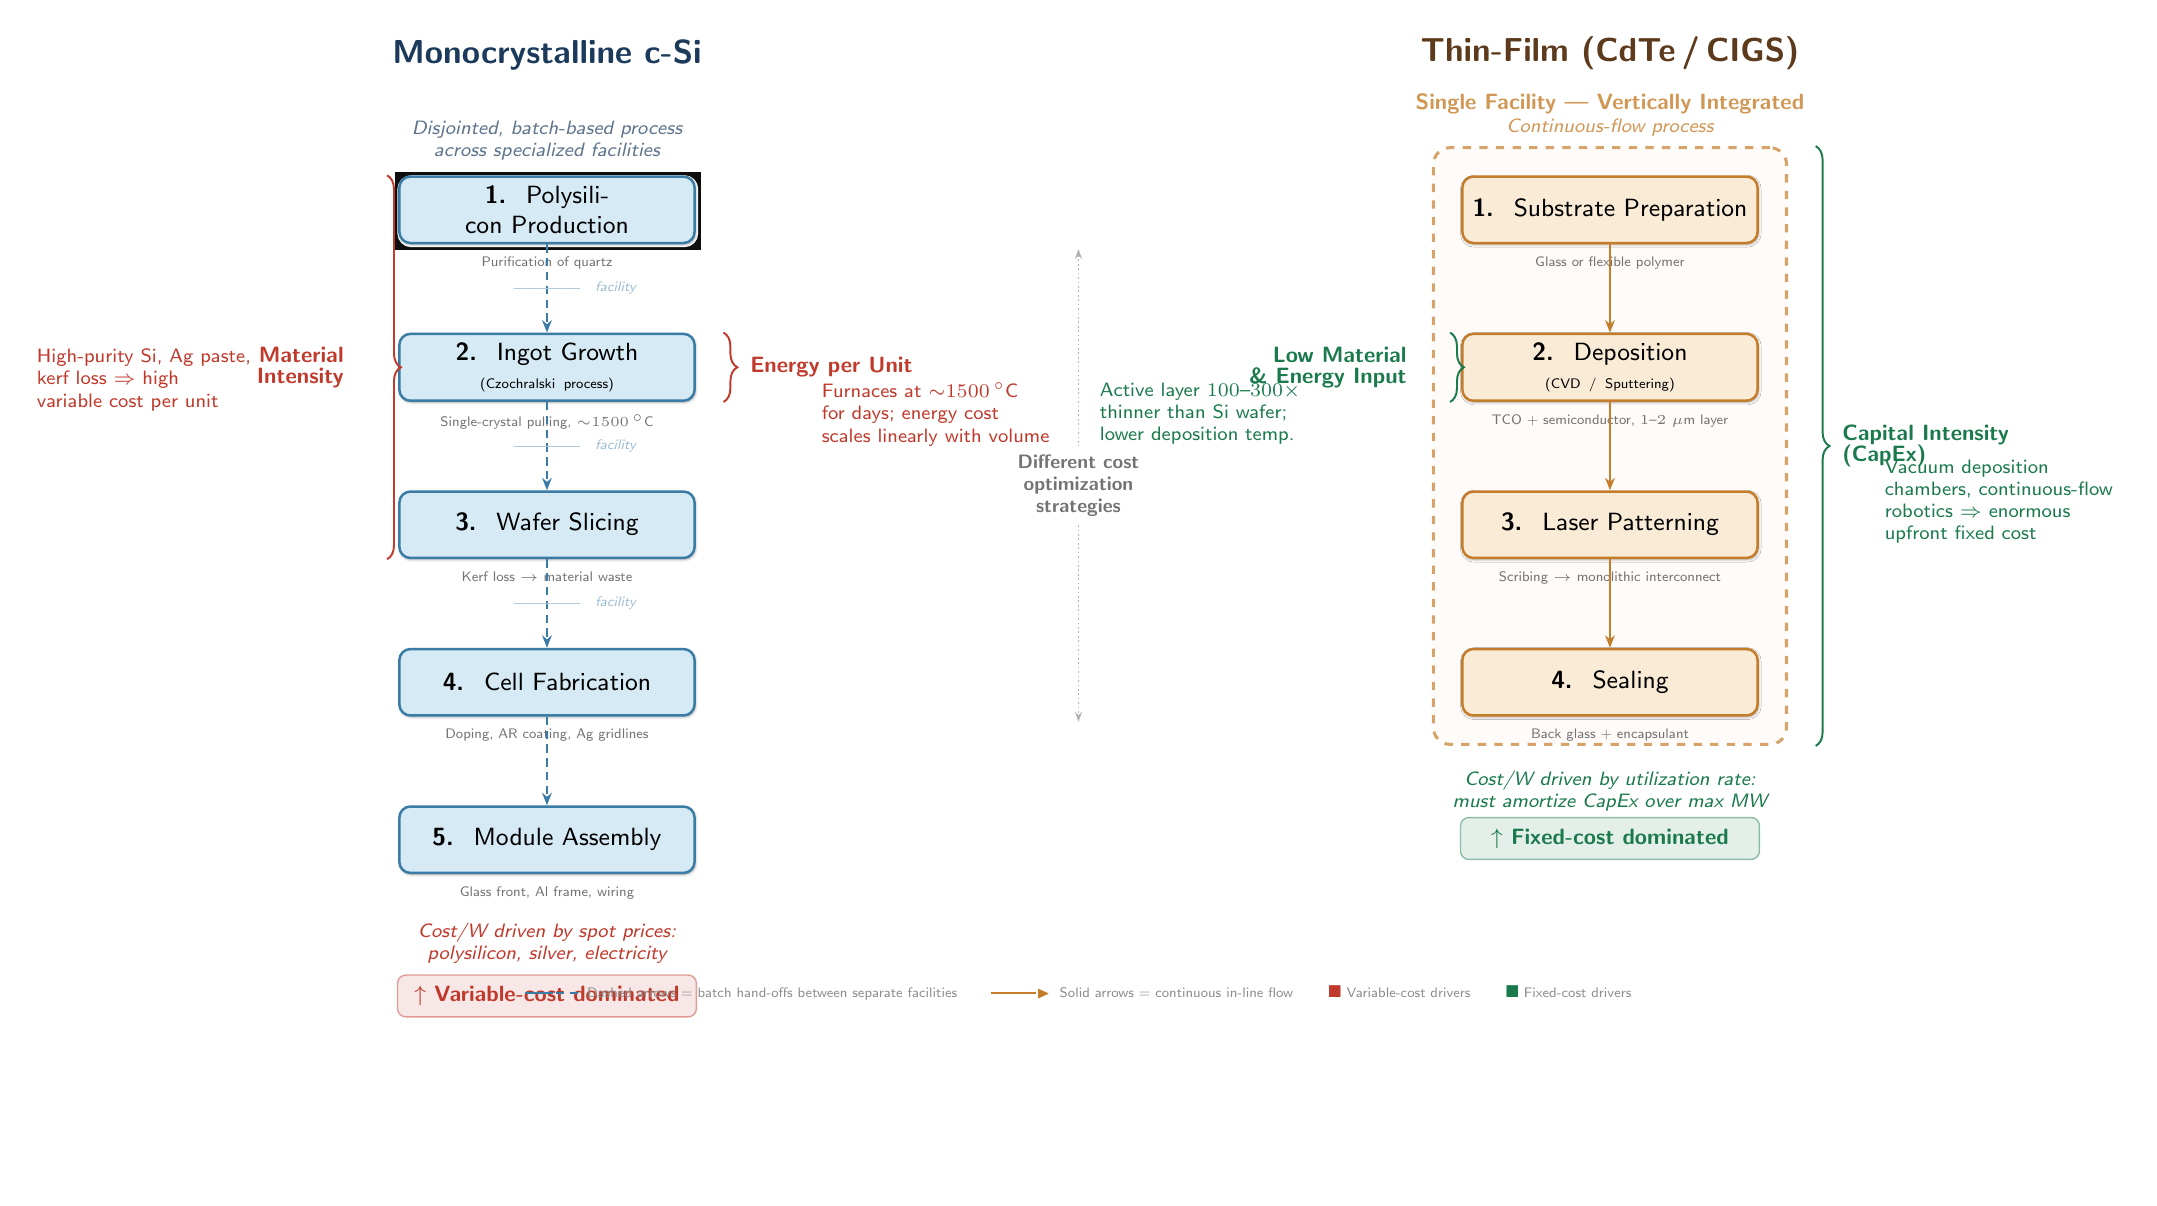
\begin{tikzpicture}[
  stage mono/.style={
    rectangle, rounded corners=4pt,
    draw=monoStage, line width=0.9pt,
    fill=monoLight,
    text width=10em, minimum height=2.4em,
    align=center, font=\sffamily\small,
    blur shadow={shadow blur steps=4, shadow xshift=0.3pt,
                 shadow yshift=-0.5pt, shadow blur radius=1pt}
  },
  stage tf/.style={
    rectangle, rounded corners=4pt,
    draw=tfStage, line width=0.9pt,
    fill=tfLight,
    text width=10em, minimum height=2.4em,
    align=center, font=\sffamily\small,
    blur shadow={shadow blur steps=4, shadow xshift=0.3pt,
                 shadow yshift=-0.5pt, shadow blur radius=1pt}
  },
  heading/.style={
    font=\sffamily\bfseries\large, anchor=south
  },
  subtitle/.style={
    font=\sffamily\itshape\scriptsize, anchor=north,
    text width=12em, align=center
  },
  detail/.style={
    font=\sffamily\tiny, text=black!55, align=center
  },
  annot/.style={
    font=\sffamily\scriptsize, align=left
  },
  arrow main/.style={
    -{Stealth[length=4.5pt,width=3.5pt]}, line width=1pt
  },
  brace style/.style={
    decorate, decoration={brace, amplitude=5pt, raise=3pt},
    line width=0.7pt, draw=bracketGray
  },
  brace label/.style={
    font=\sffamily\footnotesize\bfseries, midway
  },
  integration box/.style={
    rectangle, rounded corners=6pt, dashed, line width=1.1pt
  }
]
 
% ── Layout constants ─────────────────────────────────────────
\def\ystep{2.0cm}
\def\monoX{0}
\def\tfX{13.5}
 
% ── Background panels ────────────────────────────────────────
\begin{scope}[on background layer]
  \fill[bgLeft, rounded corners=8pt]
    (-4.8, 2.0) rectangle (5.0, -12.3);
  \fill[bgRight, rounded corners=8pt]
    (8.5, 2.0) rectangle (18.3, -12.3);
\end{scope}
 
% ══════════════════════════════════════════════════════════════
%  LEFT COLUMN — MONOCRYSTALLINE c-Si
% ══════════════════════════════════════════════════════════════
\node[heading, color=monoHead] at (\monoX, 1.65) {Monocrystalline c-Si};
\node[subtitle, color=monoHead!70] at (\monoX, 1.25)
  {Disjointed, batch-based process\\across specialized facilities};
 
\node[stage mono] (m1) at (\monoX, 0)
  {\textbf{1.}\; Polysilicon Production};
\node[detail, below=1pt of m1] {Purification of quartz};
 
\node[stage mono] (m2) at (\monoX, -\ystep)
  {\textbf{2.}\; Ingot Growth\\[-1pt]{\tiny(Czochralski process)}};
\node[detail, below=1pt of m2] {Single-crystal pulling, ${\sim}1500\,^{\circ}$C};
 
\node[stage mono] (m3) at (\monoX, -2*\ystep)
  {\textbf{3.}\; Wafer Slicing};
\node[detail, below=1pt of m3] {Kerf loss $\rightarrow$ material waste};
 
\node[stage mono] (m4) at (\monoX, -3*\ystep)
  {\textbf{4.}\; Cell Fabrication};
\node[detail, below=1pt of m4] {Doping, AR coating, Ag gridlines};
 
\node[stage mono] (m5) at (\monoX, -4*\ystep)
  {\textbf{5.}\; Module Assembly};
\node[detail, below=1pt of m5] {Glass front, Al frame, wiring};
 
% ── Dashed arrows (batch hand-offs) ─────────────────────────
\foreach \a/\b in {m1/m2, m2/m3, m3/m4, m4/m5}{
  \draw[arrow main, monoStage, densely dashed] (\a.south) -- (\b.north);
}
 
% ── Facility boundary ticks ──────────────────────────────────
\foreach \a/\b in {m1/m2, m2/m3, m3/m4}{
  \coordinate (mid) at ($(\a.south)!0.5!(\b.north)$);
  \draw[monoStage!40, line width=0.4pt]
    ([xshift=-12pt]mid) -- ([xshift=12pt]mid);
  \node[font=\sffamily\tiny, color=monoStage!50, anchor=west]
    at ([xshift=14pt]mid) {\textit{facility}};
}
 
% ── Variable-cost brace: Material Intensity (stages 1--3) ───
\draw[brace style, varColor]
  ([xshift=-7pt]m1.north west) -- ([xshift=-7pt]m3.south west)
  node[brace label, left=9pt, text=varColor, text width=7em, align=right]
  {\raggedleft Material\\[-2pt]Intensity};
 
\node[annot, text=varColor, anchor=north east, text width=8.5em]
  at ([xshift=-42pt, yshift=10pt]m2.west)
  {High-purity Si, Ag paste,\\kerf loss $\Rightarrow$ high\\variable cost per unit};
 
% ── Variable-cost brace: Energy per Unit (stage 2) ──────────
\draw[brace style, varColor]
  ([xshift=7pt]m2.north east) -- ([xshift=7pt]m2.south east)
  node[brace label, right=9pt, text=varColor, text width=7.5em, align=left]
  {Energy per Unit};
 
\node[annot, text=varColor, anchor=north west, text width=8.5em]
  at ([xshift=42pt, yshift=-2pt]m2.east)
  {Furnaces at ${\sim}1500\,^{\circ}$C\\for days; energy cost\\scales linearly with volume};
 
% ── Bottom summary (mono) ───────────────────────────────────
\node[annot, text=varColor, anchor=north, text width=12em, align=center,
      font=\sffamily\scriptsize\itshape]
  at ([yshift=-14pt]m5.south)
  {Cost/W driven by spot prices:\\polysilicon, silver, electricity};
 
\node[rectangle, rounded corners=3pt,
      fill=varColor!12, draw=varColor!50, line width=0.5pt,
      font=\sffamily\footnotesize\bfseries, text=varColor,
      inner sep=4pt, text width=10em, align=center]
  (monoSummary) at ([yshift=-44pt]m5.south)
  {$\uparrow$ Variable-cost dominated};
 
 
% ══════════════════════════════════════════════════════════════
%  RIGHT COLUMN — THIN-FILM (CdTe / CIGS)
% ══════════════════════════════════════════════════════════════
\node[heading, color=tfHead] at (\tfX, 1.65)
  {Thin-Film (CdTe\,/\,CIGS)};
 
\node[stage tf] (t1) at (\tfX, 0)
  {\textbf{1.}\; Substrate Preparation};
\node[detail, below=1pt of t1] {Glass or flexible polymer};
 
\node[stage tf] (t2) at (\tfX, -\ystep)
  {\textbf{2.}\; Deposition\\[-1pt]{\tiny(CVD / Sputtering)}};
\node[detail, below=1pt of t2]
  {TCO + semiconductor, $1$--$2\;\mu$m layer};
 
\node[stage tf] (t3) at (\tfX, -2*\ystep)
  {\textbf{3.}\; Laser Patterning};
\node[detail, below=1pt of t3]
  {Scribing $\rightarrow$ monolithic interconnect};
 
\node[stage tf] (t4) at (\tfX, -3*\ystep)
  {\textbf{4.}\; Sealing};
\node[detail, below=1pt of t4] {Back glass + encapsulant};
 
% ── Solid arrows (continuous flow) ───────────────────────────
\foreach \a/\b in {t1/t2, t2/t3, t3/t4}{
  \draw[arrow main, tfStage] (\a.south) -- (\b.north);
}
 
% ── Vertical-integration box ─────────────────────────────────
\begin{scope}[on background layer]
  \node[integration box, draw=tfStage!70, fill=tfLight!18,
        inner sep=10pt, fit=(t1)(t2)(t3)(t4)]
    (intBox) {};
  \node[font=\sffamily\footnotesize, text=tfStage!80,
        align=center, anchor=south]
    at (intBox.north)
    {\textbf{Single Facility --- Vertically Integrated}\\[-1pt]
     {\scriptsize\itshape Continuous-flow process}};
\end{scope}
 
% ── Fixed-cost brace: CapEx (all stages, right side) ────────
\draw[brace style, fixColor]
  ([xshift=7pt]intBox.north east) -- ([xshift=7pt]intBox.south east)
  node[brace label, right=9pt, text=fixColor, text width=7.5em, align=left]
  {Capital Intensity\\[-2pt](CapEx)};
 
\node[annot, text=fixColor, anchor=north west, text width=8.5em]
  at ([xshift=42pt, yshift=-30pt]t2.east)
  {Vacuum deposition\\chambers, continuous-flow\\robotics $\Rightarrow$ enormous\\upfront fixed cost};
 
% ── Fixed-cost brace: Low material/energy (stage 2, left) ───
\draw[brace style, fixColor]
  ([xshift=-7pt]t2.north west) -- ([xshift=-7pt]t2.south west)
  node[brace label, left=9pt, text=fixColor, text width=7.5em, align=right]
  {\raggedleft Low Material\\[-2pt]\& Energy Input};
 
\node[annot, text=fixColor, anchor=north east, text width=8.5em]
  at ([xshift=-42pt, yshift=-2pt]t2.west)
  {Active layer $100$--$300\times$\\thinner than Si wafer;\\lower deposition temp.};
 
% ── Bottom summary (thin-film) ──────────────────────────────
\node[annot, text=fixColor, anchor=north, text width=12em, align=center,
      font=\sffamily\scriptsize\itshape]
  at ([yshift=-16pt]t4.south)
  {Cost/W driven by utilization rate:\\must amortize CapEx over max MW};
 
\node[rectangle, rounded corners=3pt,
      fill=fixColor!12, draw=fixColor!50, line width=0.5pt,
      font=\sffamily\footnotesize\bfseries, text=fixColor,
      inner sep=4pt, text width=10em, align=center]
  (tfSummary) at ([yshift=-44pt]t4.south)
  {$\uparrow$ Fixed-cost dominated};
 
 
% ══════════════════════════════════════════════════════════════
%  CENTRE — comparison connector
% ══════════════════════════════════════════════════════════════
\coordinate (ctrTop) at ($(m1.east)!0.5!(t1.west) + (0, -0.5)$);
\coordinate (ctrBot) at ($(m5.east)!0.5!(t4.west) + (0, 0.5)$);
 
\draw[line width=0.6pt, color=black!30, densely dotted,
      {Stealth[length=3.5pt]}-{Stealth[length=3.5pt]}]
  (ctrTop) -- (ctrBot)
  node[midway, fill=white, inner sep=3pt,
       font=\sffamily\scriptsize\bfseries, text=black!55,
       text width=5.5em, align=center]
  {Different cost\\optimization\\strategies};
 
% ── Legend ────────────────────────────────────────────────────
\node[anchor=north, font=\sffamily\tiny, text=black!45,
      text width=19cm, align=center]
  at ($(monoSummary)!0.5!(tfSummary) + (0,-0.75)$)
  {%
    \textcolor{monoStage}{\rule[0.5ex]{10pt}{0.8pt}\kern1pt%
      \rule[0.5ex]{3pt}{0.8pt}\kern2pt%
      \rule[0.5ex]{3pt}{0.8pt}}
    \;Dashed arrows = batch hand-offs between separate facilities
    \qquad
    \textcolor{tfStage}{\rule[0.5ex]{16pt}{0.8pt}$\blacktriangleright$}
    \;Solid arrows = continuous in-line flow
    \qquad
    \textcolor{varColor}{$\blacksquare$}\;Variable-cost drivers
    \qquad
    \textcolor{fixColor}{$\blacksquare$}\;Fixed-cost drivers%
  };
 
\end{tikzpicture}
\end{document}